\section{Задача 1.31}
\subsection{Задание:}
Вычислить
$
	\begin{vmatrix}
		1 & 2 & 3 & \cdots & n - 1 & n \\
		-1 & 0 & 3 & \cdots & n - 1 &  n \\
		-1 & -2 & 0 & \cdots & n - 1 & n \\
		\vdots & \vdots & \vdots & \ddots & \vdots & \vdots \\
		-1 & -2 & -3 & \cdots & -(n - 1) & 0 \\
	\end{vmatrix}
$.
\subsection{Решение:}
Вынесем общий множитель из каждого столбца определителя (вынесем из каждого столбца номер этого столбца),
тогда определитель принимает вид:
\\[1em]
$
	n! \cdot
	\begin{vmatrix}
		1 & 1 & 1 & \cdots & 1 & 1 \\
		-1 & 0 & 1 & \cdots & 1 &  1 \\
		-1 & -1 & 0 & \cdots & 1 & 1 \\
		\vdots & \vdots & \vdots & \ddots & \vdots & \vdots \\
		-1 & -1 & -1 & \cdots & -1 & 0 \\
	\end{vmatrix}
$
\\[1em]
Докажем методом мат. индукции что
$
	\begin{vmatrix}
		1 & 1 & 1 & \cdots & 1 & 1 \\
		-1 & 0 & 1 & \cdots & 1 &  1 \\
		-1 & -1 & 0 & \cdots & 1 & 1 \\
		\vdots & \vdots & \vdots & \ddots & \vdots & \vdots \\
		-1 & -1 & -1 & \cdots & -1 & 0 \\
	\end{vmatrix}
	= 1
$
\\[1em]
Проверим базу $ n = 1 $: $ |1| = 1 $
\\
Предположим что утверждение верно для $ n $, тогда докажем для $ n + 1 $:
\\[1em]
$
	\begin{vmatrix}
		1 & 1 & 1 & \cdots & 1 & 1 \\
		-1 & 0 & 1 & \cdots & 1 &  1 \\
		-1 & -1 & 0 & \cdots & 1 & 1 \\
		\vdots & \vdots & \vdots & \ddots & \vdots & \vdots \\
		-1 & -1 & -1 & \cdots & -1 & 0 \\
	\end{vmatrix}_{n + 1}
	=
	\begin{vmatrix}
		1 & 1 & 1 & \cdots & 1 & 1 \\
		-1 & 0 & 1 & \cdots & 1 &  1 \\
		-1 & -1 & 0 & \cdots & 1 & 1 \\
		\vdots & \vdots & \vdots & \ddots & \vdots & \vdots \\
		0 & 0 & 0 & \cdots & 0 & 1 \\
	\end{vmatrix}_{n + 1}
	=
	1 \cdot
	\begin{vmatrix}
		1 & 1 & 1 & \cdots & 1 & 1 \\
		-1 & 0 & 1 & \cdots & 1 &  1 \\
		-1 & -1 & 0 & \cdots & 1 & 1 \\
		\vdots & \vdots & \vdots & \ddots & \vdots & \vdots \\
		-1 & -1 & -1 & \cdots & -1 & 0 \\
	\end{vmatrix}_{n}
$
\\[1em]
Утверждение доказано.
\\[1em]
Получается что
$
	\begin{vmatrix}
		1 & 2 & 3 & \cdots & n - 1 & n \\
		-1 & 0 & 3 & \cdots & n - 1 &  n \\
		-1 & -2 & 0 & \cdots & n - 1 & n \\
		\vdots & \vdots & \vdots & \ddots & \vdots & \vdots \\
		-1 & -2 & -3 & \cdots & -(n - 1) & 0 \\
	\end{vmatrix}
	=
	n!
$
\subsection{Компьютерная проверка:}
Выполним проверку в среде Wolfram Mathematica при $ n = 8 $:
\\
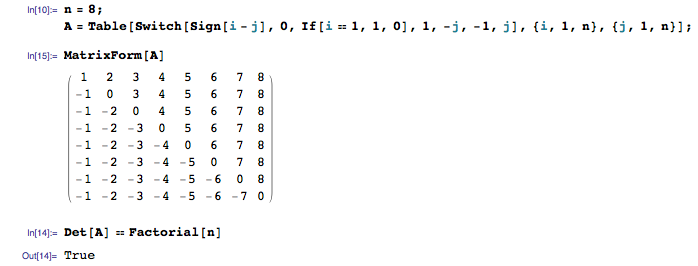
\includegraphics[scale=0.6]{task/1_31/screen1.png}
\subsection{Вывод:}
Компьютерная проверка подтвертила правильность полученной формулы.
